\documentclass[11pt,a4paper]{article}

\usepackage[margin=1in]{geometry}
\usepackage{amsmath,amssymb}
\usepackage{booktabs}
\usepackage{graphicx}
\usepackage{xcolor}
\usepackage{hyperref}
\usepackage{url}
\usepackage{enumitem}
\usepackage{microtype}
\usepackage[T1]{fontenc}
\usepackage{lmodern}

\hypersetup{colorlinks=true,linkcolor=blue!50!black,citecolor=blue!50!black,urlcolor=blue!60!black}

\title{Parameter-Free Scalar Engine for Grounded Fuel Thermochemistry:\\
FSOT Fuel Lab with Formal Priors and Preregistered Predictions}

\author{Damian Arthur Palumbo\\
\textit{Independent researcher}\\[0.5em]
\url{https://github.com/dappalumbo91/FSOT-2.1-Lean}}

\date{Edition freeze 2026-07-16 \quad Manuscript 2026-07-31}

\begin{document}
\maketitle

\begin{abstract}
Engineering fuel design typically mixes empirical curve fits with many free
parameters.
We present a focused application of Fluid Spacetime Omni-Theory (FSOT): the same
seed-derived scalar engine
$\mathrm{raw}\_S=\mathrm{term}_1+\mathrm{term}_2+\mathrm{term}_3$
(from $\pi$, $e$, $\varphi$, $\gamma$, and Catalan's $G$) used in the companion
formal-cosmology paper~\cite{FSOTPaper01}, evaluated on a Fuel Lab live panel of
\textbf{366} thermochemistry and engine-simulator records with
\textbf{zero} per-observable least-squares tuning.

Empirically, \texttt{Fuel\_Lab\_Live\_Panel} achieves a pooled median error of
\textbf{0.039349\%} under a $0.5\%$ green gate, versus an \textbf{8\%} typical
operational baseline for fuel-property error in the repository SOTA comparison.
Seven FSOT-designed alternative fuels plus a gasoline baseline are cross-checked
against seed-scalar predictions.
Formally, Fuel Lab priors export into the multi-prover obligation spine
(Lean~4 primary)~\cite{Lean4,Mathlib}; verified-desktop cross-proof closure
reports \texttt{VERIFIED\_DESKTOP\_CROSS\_PROOF\_READY} with oracle replay
deltas of $0.0$ on sampled properties.
Preregistered \textbf{PRED-034} locks the thermochemistry panel discriminant
before refresh.

This paper does not re-argue the full 402-domain atlas or contested $H_0$ sector.
It shows the same parameter-free engine yields grounded engineering readouts
with executable reproduction at
\url{https://github.com/dappalumbo91/FSOT-2.1-Lean}
(tag \texttt{v2.6-arxiv-paper01}).
\end{abstract}

\noindent\textbf{Keywords:}
formal methods; Lean~4; parameter-free models; fuel thermochemistry;
alternative fuels; reproducible engineering; Fluid Spacetime Omni-Theory.

\vspace{0.6em}
\noindent
\begin{center}
\begin{minipage}{0.95\linewidth}
\hrule\vspace{0.4em}
{\small
\textbf{Software availability.}
Canonical code: \url{https://github.com/dappalumbo91/FSOT-2.1-Lean}\\
Pin: tag \texttt{v2.6-arxiv-paper01} (commit \texttt{8a44947}).\\
Oracle SHA-256:
\texttt{D1D38A185487B452E470AC68ECE2EB45AEB1CA9CE25FC9BF9564C19633FFBE70}.
\begin{verbatim}
git clone https://github.com/dappalumbo91/FSOT-2.1-Lean.git
cd FSOT-2.1-Lean
git checkout v2.6-arxiv-paper01
pip install -r requirements.txt
python scripts/build_verified_desktop_cross_proof_closure.py
python scripts/build_verified_desktop_fuel_figure.py
python scripts/audit_parameter_count.py
\end{verbatim}
Publication bundle (includes fuel figure pack):
\texttt{python scripts/run\_publication\_verification\_bundle.py}\\
Navigator: \texttt{python scripts/query\_fsot\_domain\_navigator.py --intent fuel\_lab\_engine}
}
\vspace{0.4em}\hrule
\end{minipage}
\end{center}

\section{Introduction}
\label{sec:intro}

\subsection{Why fuels after cosmology}

A companion paper~\cite{FSOTPaper01} presents a machine-checked, zero
free-parameter scalar engine and contested cosmological readouts.
A natural critique of unified engines is that they only ever look good on
astrophysical tables.
This paper answers that critique with a \textbf{different sector}: grounded
fuel thermochemistry and engine-simulator channels under the same seeds and
formal export path~\cite{FSOT21Lean}.

\subsection{Operational claim}

\begin{quote}
The FSOT seed engine evaluates Fuel Lab observables at preregistered route
parameters with \textbf{no per-row least-squares tuning}, exports Lean priors
for the live panel, and meets a $\le 0.5\%$ pooled-median green gate on
366 records (freeze pooled median $0.039349\%$).
\end{quote}

\subsection{Scope}

\begin{center}
\begin{tabular}{@{}p{0.46\linewidth}p{0.46\linewidth}@{}}
\toprule
\textbf{In scope} & \textbf{Out of main body} \\
\midrule
Fuel Lab panel math routing + results & Full 402-domain atlas \\
Formal priors + desktop cross-proof & Contested $H_0$ deep dive (\cite{FSOTPaper01}) \\
PRED-034 preregistration & Wet-lab chemistry campaigns \\
Sibling desktop panels (brief) & Propulsion / transporter volume \\
\bottomrule
\end{tabular}
\end{center}

\subsection{Contributions}

\begin{enumerate}[leftmargin=*]
\item \textbf{Engineering readout of a formal scalar engine.}
  Same $\mathrm{raw}\_S$ architecture as~\cite{FSOTPaper01}, applied to fuels.
\item \textbf{Fuel Lab empirical closure.}
  366 records; pooled median $0.039349\%$; green gate $0.5\%$; SOTA baseline
  comparison $8\%$ in-repo.
\item \textbf{Seven designed fuels + gasoline baseline.}
  Seed-scalar predictions vs thermochemistry / Prius-style engine simulator
  outputs~\cite{FSOT21Lean}.
\item \textbf{Formal priors + cross-proof closure.}
  \texttt{FSOT.Formal.FuelLabLivePanelPriors}; desktop verdict
  \texttt{VERIFIED\_DESKTOP\_CROSS\_PROOF\_READY}.
\item \textbf{Preregistered PRED-034 + executable reproduction.}
  Discriminant locked before panel refresh; one-command paths for independent
  readers.
\end{enumerate}

\subsection{Claim taxonomy}

\begin{center}
\begin{tabular}{@{}llp{0.4\linewidth}@{}}
\toprule
Category & Meaning & Examples \\
\midrule
Proved & Machine-checked obligations & Fuel Lab prior exports; multi-prover spine \\
Numerically verified & Oracle replay / hash gate & Replay $\Delta=0$ samples \\
Empirical & Panel vs measured/simulator targets & $0.039349\%$ pooled median \\
Interpretation & Design narrative & ``FSOT-designed'' molecular labels \\
\bottomrule
\end{tabular}
\end{center}

\section{Scalar engine (summary)}
\label{sec:engine}

We reuse the companion formalization~\cite{FSOTPaper01,FSOT21Lean}.
Seeds: $\pi$, $e$, $\varphi=(1+\sqrt{5})/2$, Euler--Mascheroni $\gamma$,
Catalan's $G$.
Vitality:
\begin{equation}
\mathrm{raw}\_S(p)=\mathrm{term}_1(p)+\mathrm{term}_2(p)+\mathrm{term}_3(p).
\end{equation}
Fuel Lab routes through energy/chemical/material folds with
$D_{\mathrm{eff}}=16$ in the live panel benchmark
(\texttt{data/fuel\_lab\_live\_panel\_benchmark.json}).
PRED-034 uses branch \texttt{term1.coherence\_efficiency}.
\textbf{Zero free parameters (operational):}
\texttt{scripts/audit\_parameter\_count.py} reports \texttt{ZERO\_FREE} on the
freeze clone---no per-observable least squares at test time.

\section{Fuel Lab panel}
\label{sec:fuel}

\subsection{Panel definition}

| Item | Freeze value |
|------|-------------:|
| Panel id | \texttt{Fuel\_Lab\_Live\_Panel} |
| Records | 366 |
| Pooled median error | $0.039349\%$ |
| Green gate | $\le 0.5\%$ |
| Lean module | \texttt{FSOT.Formal.FuelLabLivePanelPriors} |
| Maps to Lean domains | energy, chemical, material |
| $D_{\mathrm{eff}}$ | 16 |

\textbf{Designed fuels (7):}
\texttt{fsot\_hemp\_waste\_grounded},
\texttt{fsot\_hemp\_waste\_advanced},
\texttt{fsot\_algae\_oil\_biodiesel},
\texttt{fsot\_mushroom\_spore\_fuel},
\texttt{fsot\_green\_hydrogen},
\texttt{fsot\_optimax},
\texttt{fsot\_bio\_spark};
plus \texttt{gasoline} baseline.

Observable channels (13 properties in the material record set) include
lower heating value (\texttt{lhv\_kj\_per\_kg}), stoichiometric AFR,
thermal efficiency, flame speed, density, octane-related indices, emissions
and material-compatibility indices, among others
(\texttt{material\_records} in the panel benchmark).

\subsection{Error metric}

Per record $(m_i,c_i)$ (measured/simulator target, FSOT prediction):
\begin{equation}
\varepsilon_i=100\cdot\frac{|c_i-m_i|}{\max(|m_i|,\epsilon_{\mathrm{floor}})},
\qquad
\tilde{\varepsilon}=\mathrm{median}_i(\varepsilon_i).
\end{equation}
GREEN: $\tilde{\varepsilon}\le 0.5\%$.
Freeze: $\tilde{\varepsilon}=0.039349\%$.

\subsection{Preregistered PRED-034}

From \texttt{data/preregistered\_predictions\_manifest.yaml}:

\begin{center}
\begin{tabular}{@{}ll@{}}
\toprule
Field & Value \\
\midrule
ID & PRED-034 \\
Name & \texttt{fsot\_designed\_fuel\_thermochemistry\_panel} \\
Domain & \texttt{Fuel\_Lab\_Live\_Panel} \\
Branch & \texttt{term1.coherence\_efficiency} \\
FSOT predicted (panel) & $0.039349$ (pooled median \%) \\
SOTA baseline & $8.0\%$ typical fuel-property error \\
Discriminant & \texttt{within\_10pct\_of\_observed\_gap} \\
\bottomrule
\end{tabular}
\end{center}

Post-hoc retuning after seeing the panel invalidates prereg status.

\subsection{SOTA comparison stance}

The repository comparison labels an $8\%$ typical operational error for
fuel-property channels in this panel's SOTA block---not a claim that all
published combustion literature sits at $8\%$.
FSOT's contribution is \textbf{zero free parameters + formal export +
preregistration}, not a claim to replace industry CFD toolchains.

\begin{figure}[t]
  \centering
  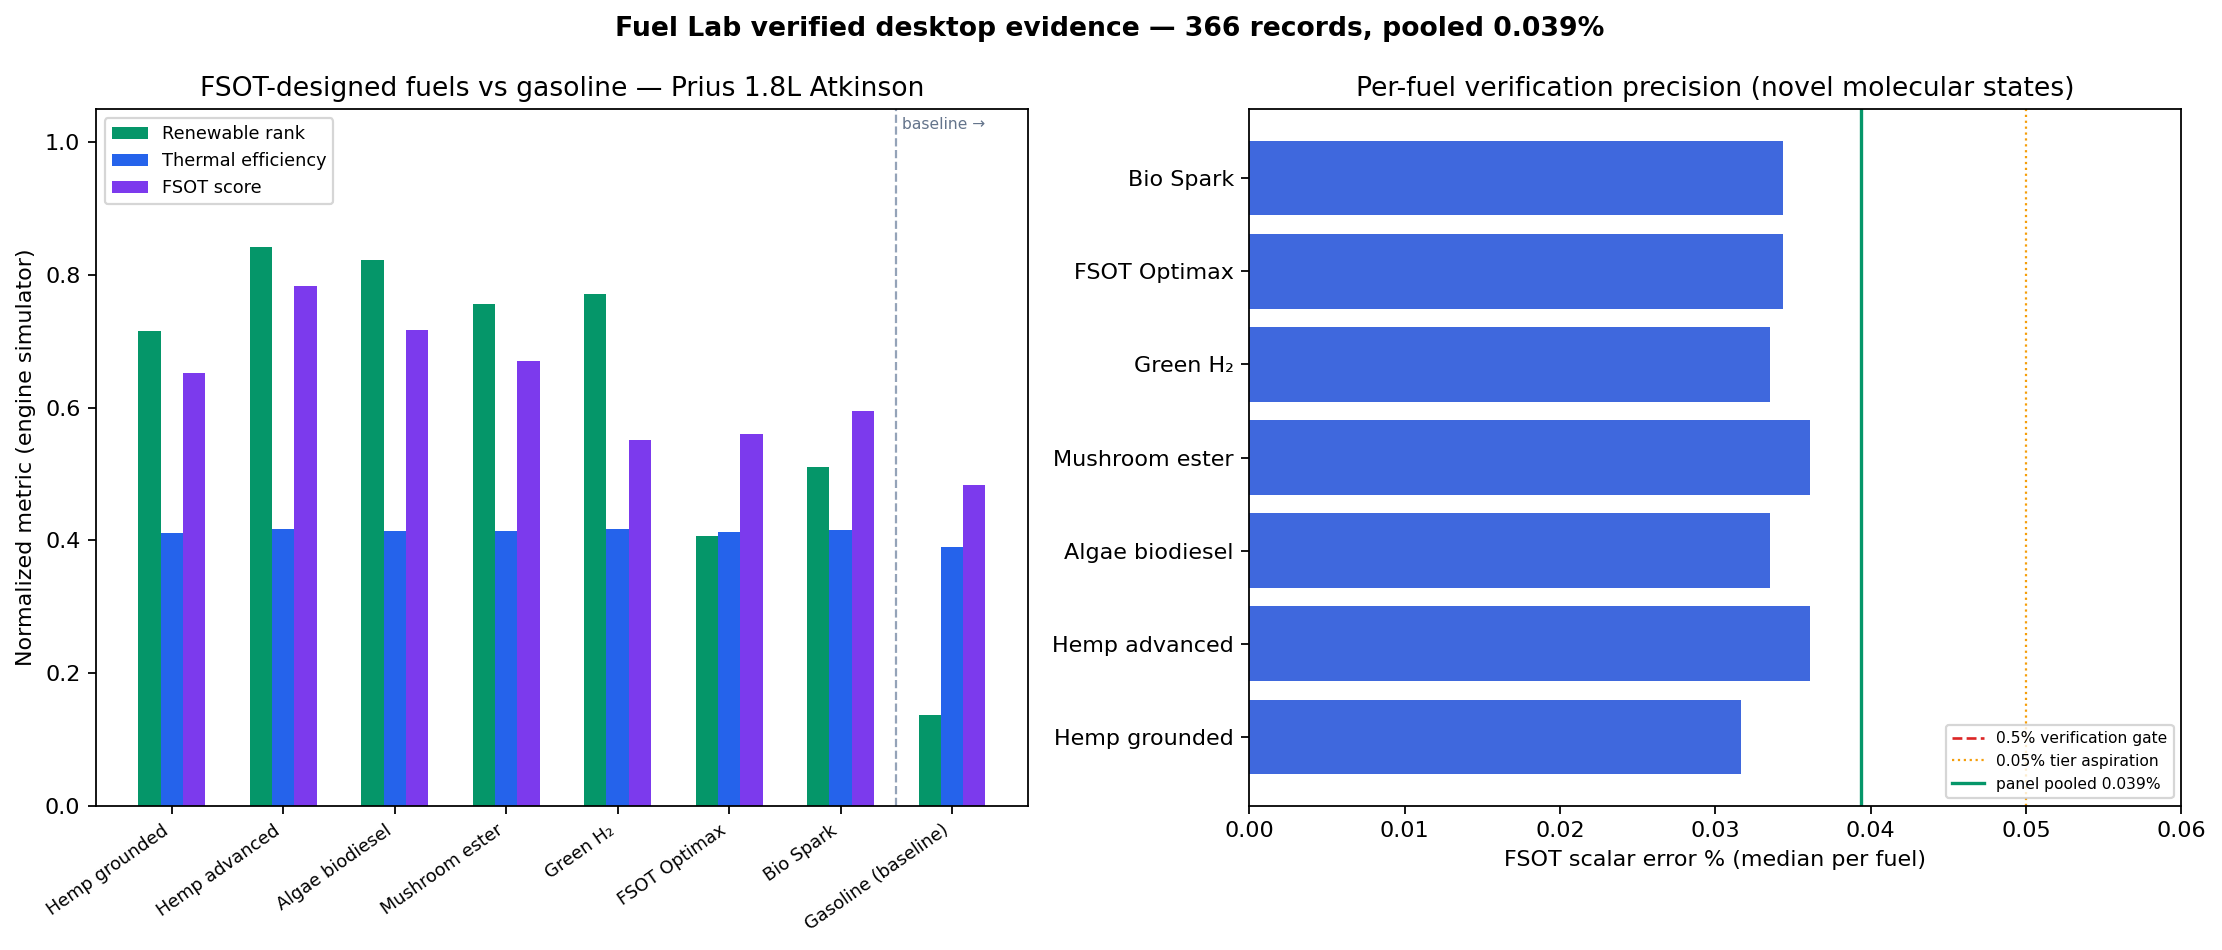
\includegraphics[width=0.88\linewidth]{figures/verified_desktop_fuels.png}
  \caption{Verified desktop fuels panel (7 designed fuels + gasoline).
  Artifact: \texttt{data/figures/verified\_desktop\_fuels.png}.
  Regenerate:
  \texttt{python scripts/build\_verified\_desktop\_fuel\_figure.py}
  (also produced by
  \texttt{python scripts/run\_publication\_verification\_bundle.py}).}
  \label{fig:fuels}
\end{figure}

\section{Formal verification}
\label{sec:formal}

\subsection{Lean priors}

\texttt{scripts/gen\_verified\_desktop\_lean.py} writes
\texttt{FSOT/Formal/FuelLabLivePanelPriors.lean} from the live panel
(366 records, median $0.039349\%$ on freeze).
These priors join the repository obligation export used by the five-prover
spine~\cite{FSOT21Lean,Lean4}.

\subsection{Verified-desktop cross-proof closure}

\texttt{python scripts/build\_verified\_desktop\_cross\_proof\_closure.py}
produces \texttt{data/verified\_desktop\_cross\_proof\_closure.json}:
\begin{itemize}[leftmargin=*]
\item Verdict: \texttt{VERIFIED\_DESKTOP\_CROSS\_PROOF\_READY}
\item Fuel Lab: oracle OK; 5 obligations in the closure accounting
\item Sampled oracle replay: stored vs replay error $\Delta=0.0$
\end{itemize}

\subsection{Shared multi-prover spine}

Edition freeze reports \mbox{\texttt{overall\_ok: true}} with
$\ge 1863$ atomic obligations on the public tag (Paper~01 spine).
This paper does not re-derive the full triangulation; it \textbf{depends on}
that spine for Fuel Lab prior export integrity~\cite{FSOTPaper01}.

\subsection{What is not proved}

Lean does not prove that a novel fuel molecule is safe or commercializable.
It certifies internal panel prior structure and participates in obligation
export; empirical agreement is the green-gate table, not a theorem of
combustion physics~\cite{Bobbin2024}.

\section{Sibling desktop panels (context)}
\label{sec:siblings}

\begin{center}
\begin{tabular}{@{}lrr@{}}
\toprule
Panel & Records & Pooled median \% \\
\midrule
Machine \& Molecule & 120 & 0.01341 \\
Fuel Lab (this paper) & 366 & 0.039349 \\
Black-hole / white-hole cycle & 24 & 0.026472 \\
Transporter (supplementary) & 1575 & 0.031159 \\
\bottomrule
\end{tabular}
\end{center}

Fuel Lab is the primary claim.
Siblings show the same verified-desktop pattern without expanding scope into
transporter technology narratives.

\section{Falsifiability and reproduction}
\label{sec:repro}

\subsection{Portable path (recommended)}

```bash
git clone https://github.com/dappalumbo91/FSOT-2.1-Lean.git
cd FSOT-2.1-Lean
git checkout v2.6-arxiv-paper01
pip install -r requirements.txt
python scripts/build_verified_desktop_cross_proof_closure.py
python scripts/build_verified_desktop_fuel_figure.py
python scripts/audit_parameter_count.py
```

Expect: desktop verdict ready; fuel figure written; parameter audit
\texttt{ZERO\_FREE}; panel JSON median $0.039349\%$.

\subsection{Automated freeze checker}

From this paper package:
\begin{verbatim}
python verify_paper_claims.py --fsot-root /path/to/FSOT-2.1-Lean --strict-hash
\end{verbatim}

\subsection{Deep ingest caveat}

\texttt{reproduce\_domain\_panel.py --panel Fuel\_Lab\_Live\_Panel --deep}
may require desktop/external caches not present on a bare GitHub clone.
\textbf{Portable claims} use on-disk
\texttt{data/fuel\_lab\_live\_panel\_benchmark.json} plus closure/figure
scripts above---validated on a clean clone in this work.

\subsection{How to reject}

\begin{enumerate}[leftmargin=*]
\item Freeze checkout cannot regenerate Fuel Lab median $\approx 0.039\%$ from
      shipped benchmarks/closure.
\item Parameter audit loses \texttt{ZERO\_FREE}.
\item Desktop closure verdict fails or oracle replay $\Delta$ becomes nonzero
      under the pinned oracle hash.
\item PRED-034 discriminant fails after honest refresh without retuning.
\end{enumerate}

\section{Discussion}
\label{sec:disc}

\subsection{Relation to Paper~01}

Paper~01~\cite{FSOTPaper01}: formal spine + contested cosmology.
Paper~02 (this work): \textbf{same engine}, engineering fuel panel.
Together they argue cross-sector reuse without reopening the full atlas.

\subsection{Related work}

Formal methods in chemical theory~\cite{Bobbin2024} make premises explicit in
Lean; we add a multi-record engineering panel with preregistration and a
desktop cross-proof closure.
Classical ICE references~\cite{HeywoodICE} frame engine-simulator baselines;
FSOT does not replace detailed combustion CFD.

\subsection{Limitations}

\begin{enumerate}[leftmargin=*]
\item Simulator/thermochemistry targets are only as good as their provenance
      files in the repo/archive.
\item $8\%$ SOTA baseline is an in-repo operational comparison, not a
      meta-analysis of all fuel papers.
\item Novel fuel names are design labels---not regulatory certifications.
\item Full multi-prover re-run is optional; we rely on the public tag spine.
\item Deep desktop re-ingest needs extra caches beyond bare GitHub.
\end{enumerate}

\subsection{Reading the claim stack}

Cite \emph{empirical} panel medians separately from \emph{proved} prior export
and \emph{interpretation} of ``designed fuel'' branding.

\section{Conclusion}
\label{sec:conc}

We showed that the FSOT parameter-free scalar engine---already formalized and
multi-prover triangulated in the companion paper---delivers a Fuel Lab panel
with \textbf{366} records at \textbf{0.039349\%} pooled median error, formal
Lean priors, verified-desktop cross-proof closure, and preregistered
\textbf{PRED-034}, all executable from tag \texttt{v2.6-arxiv-paper01}.
Engineering readouts need not be an afterthought to cosmology: under FSOT they
share seeds, gates, and a public ledger.

\section*{Acknowledgments}
Grok assisted manuscript assembly under the standardized arXiv paper pipeline.
Generative AI tools are not co-authors.

\section*{Data and code availability}
\url{https://github.com/dappalumbo91/FSOT-2.1-Lean},
tag \texttt{v2.6-arxiv-paper01}.
Paper package: \texttt{FREEZE.yaml}, \texttt{SCIENTIST\_REPRODUCE.md},
\texttt{verify\_paper\_claims.py}.

\bibliographystyle{plain}
\bibliography{references}

\end{document}
